% Charlotte Geiger - Manuel Lippert - Leonard Schatt
% Physikalisches Praktikum

% Teilauswertung 1

\section{Umkehrverstärker}


\subsection*{Verstärkung und Eingangswiderstand}
In dieser Teilaufgabe der Auswertung wird $R_1=10~\text{k}\Omega$ und $R_{2,1}=1~\text{M}\Omega$ bzw. $R_{2,2}=4.7~\text{M}\Omega$ verwendet. Nun sollten wir sowohl den Frequenzgang der Verstärkung $v$ von 10Hz ab messen, als auch die Flankenabfallszeit $\tau$ bei der Übertragung einer Rechteckspannung.\\
Zuerst berechnen wir die Verstärkung $v$ und den Eingangswiderstand $R_e$. \\
Dabei bezeichnet $v_{t1}$ die theoretische Berechnung der Verstärkung bei Nutzung des Widerstandes $R_{2,1}=1~\text{M}\Omega$, und $v_{t2}$ die theoretische Berechnung der Verstärkung mit dem Widerstand $R_{2,1}=4.7~\text{M}\Omega$. Der Eingangswiderstand ergibt sich folgendermaßen: \\
$R_e=\frac{U_e}{I_1}=R_1=10~\text{k}\Omega$
\begin{equation}
    v=-\frac{R_2}{R_1} \tab \Rightarrow \tab v_{t1}= -100, \tab v_{t2}=-470
\end{equation}
Nun folgt die Fehlerberechnung mit dem Fehlerfortpflanzungsgesetz:
\begin{gather}
    u_{v}=\sqrt{\bigl(-\frac{1}{R_1}\cdot u_{R_2}\bigr)^2 + {\bigl(\frac{R_2}{R_1^2}\cdot u_{R_1}\bigr)^2}}\\
    u_{R_e}=u_{R_1}
\end{gather}
Den Fehler für die Widerstände nehmen wir als kleiner 3 Prozent an. Daraus ergeben sich folgende theoretischen Werte:
\begin{gather}
\boxed{R_e=R_1=(10.0\pm 0.3)~\text{k}\Omega}\\
R_{2,1}=(1.00\pm 0.03)~\text{M}\Omega\\
R_{2,2}=(4.71\pm 0.14)~\text{M}\Omega\\
v_{t1}=-(100\pm4)\\
v_{t2}=-(470\pm20)
\end{gather}
Beim Versuch, die gemessene Verstärkung $v$ mit den theoretisch berechneten Werten der Verstärkung  $v_{t1}$ bzw $v_{t2}$ fällt auf, dass die theoretischen Werte nicht von der Frequenz abhängen. Beim Vergleich der Werte wird deutlich, dass die theoretisch berechnete Verstärkung die Verstärkung sehr kleiner Frequenzen beschreibt. Daher nehmen wir die gemessene Verstärkung von kleinen Frequenzen als Vergleich. 
\begin{gather}
    \boxed{v_1(f=10~\text{Hz})=(98\pm 15) \tab v_2(f=10~\text{Hz})=(460\pm 49)}
\end{gather}
Beim Vergleich erkennt man, dass die Beträge der Werte sich in den Fehlerbereichen überschneiden und daher im Rahmen der Messgenauigkeit übereinstimmen. Jedoch fällt auch auf, dass die theoretischen Werte negativ, die gemessenen jedoch positiv sind. Der Grund dafür ist die Phasenverschiebung von Eingangs und Ausgangssignal.


\subsection*{Frequenzgang und Verstärker-Bandbreiten-Produkt}
Für den Fehler des Oszilloskop wird ein Ablesefehler $s_a = 0.1~\text{Div}$ und ein Restfehler $s_r = 0.03\cdot\text{Messwert in Div}$ verwendet, woraus mit der Einstellung des Oszilloskops folgt:
\begin{gather}
    U = \text{Messwert}\cdot\text{Einstellung} = [\text{Div}]\cdot[\text{V/Div}]\\
    s_U = [\text{V/Div}]\sqrt{(0.03\cdot [\text{Div}])^2 + (0.1~[\text{Div}])^2} 
\end{gather}
Daraus folgt auch der Fehler für die Verstärkung $v$ mit dem Fehlerfortpflanzungsgesetz wie folgt:
\begin{gather}
    v = \frac{U_a}{U_e} \Rightarrow s_v = \sqrt{\left(\frac{s_{U_a}}{U_e}\right)^2 + \left(\frac{U_a s_{U_e}}{(U_e)^2}\right)^2}
\end{gather}
Mit diesen Formel ergibt sich dann Tabelle \ref{tab:1MOhm}, wobei ab Messwert 20 ein Ablesefehler von $1~\text{Div}$ (erschwertes Ablesen), und Tabelle \ref{tab:4,7MOhm}, wobei da generell ein Ablesefehler von $1~\text{Div}$ verwendet wird wegen den schwierigen Ablesebedingungen.
\newpage
\begin{center}
    \captionof{table}{Messreihe für $R_{2,1}$}
    \begin{tabular}{l | c c c c c | c c}
        {} &       $f$/Hz &  $U_a$/mV &  $s_{U_a}$/mV &  $U_e$/mV &  $s_{U_e}$/mV &   $v$ &   $s_v$ \\
        \hline
        1  &       10 &  9800 &       356 &     100 &         4 &  98.00 &  5.01 \\    
        2  &    25000 &  8000 &       312 &     100 &         4 &  80.00 &  4.25 \\    
        3  &    33300 &  7000 &       290 &     100 &         4 &  70.00 &  3.84 \\    
        4  &    40000 &  6400 &       277 &     100 &         4 &  64.00 &  3.61 \\    
        5  &    50000 &  5400 &       190 &     100 &         4 &  54.00 &  2.72 \\    
        6  &   100000 &  3050 &       136 &     100 &         4 &  30.50 &  1.75 \\    
        7  &   200000 &  1550 &        68 &     100 &         4 &  15.50 &  0.88 \\    
        8  &   300000 &  1000 &        36 &     100 &         4 &  10.00 &  0.51 \\    
        9  &   400000 &   740 &        30 &     100 &         4 &   7.40 &  0.40 \\    
        10 &   500000 &   550 &        19 &     100 &         4 &   5.50 &  0.28 \\    
        11 &   600000 &   450 &        17 &     100 &         4 &   4.50 &  0.23 \\    
        12 &   700000 &   370 &        15 &     100 &         4 &   3.70 &  0.20 \\    
        13 &   800000 &   300 &        13 &     100 &         4 &   3.00 &  0.17 \\    
        14 &   900000 &   255 &         9 &     100 &         4 &   2.55 &  0.13 \\    
        15 &  1000000 &   220 &         8 &     100 &         4 &   2.20 &  0.11 \\    
        16 &  1100000 &   190 &         8 &     100 &         4 &   1.90 &  0.10 \\    
        17 &  1200000 &   170 &         7 &     100 &         4 &   1.70 &  0.09 \\    
        18 &  1300000 &   150 &         7 &     100 &         4 &   1.50 &  0.09 \\    
        19 &  1400000 &   140 &         7 &     100 &         4 &   1.40 &  0.08 \\    
        20 &  1500000 &   120 &        50 &     100 &         4 &   1.20 &  0.50 \\    
        21 &  1600000 &   108 &        20 &     100 &         4 &   1.08 &  0.21 \\    
        22 &  1700000 &   100 &        20 &     100 &         4 &   1.00 &  0.21 \\    
        23 &  1800000 &    92 &        20 &     100 &         4 &   0.92 &  0.20 \\    
    \end{tabular}
    \label{tab:1MOhm}
    \newpage
    \captionof{table}{Messreihe für $R_{2,2}$}
    \begin{tabular}{l | c c c c c | c c}
        {} &       $f$/Hz &  $U_a$/mV &  $s_{U_a}$/mV &  $U_e$/mV &  $s_{U_e}$/mV &   $v$ &   $s_v$ \\
        \hline
        1  &        10 &  9200 &      2019 &    20 &         5 &  460.0 &  153.6 \\  
        2  &      3000 &  8700 &      2017 &    20 &         5 &  435.0 &  148.9 \\  
        3  &      4000 &  8400 &      2016 &    20 &         5 &  420.0 &  146.1 \\  
        4  &      5000 &  7600 &      2013 &    20 &         5 &  380.0 &  138.9 \\  
        5  &     10000 &  5200 &      1012 &    20 &         5 &  260.0 &   82.7 \\  
        6  &    200000 &   325 &        51 &    20 &         5 &   16.2 &    4.8 \\  
        7  &    400000 &   170 &        50 &    20 &         5 &    8.5 &    3.3 \\  
        8  &    600000 &   140 &       100 &    20 &         5 &    7.0 &    5.3 \\  
        9  &    800000 &    86 &        20 &    20 &         5 &    4.3 &    1.5 \\  
        10 &   1000000 &    72 &        20 &    20 &         5 &    3.6 &    1.4 \\  
        11 &   2000000 &    50 &        10 &    20 &         5 &    2.5 &    0.8 \\  
        12 &   3000000 &    42 &        10 &    20 &         5 &    2.1 &    0.7 \\  
        13 &   4000000 &    44 &        10 &    20 &         5 &    2.2 &    0.7 \\  
        14 &   5000000 &    40 &        10 &    20 &         5 &    2.0 &    0.7 \\  
        15 &   6000000 &    40 &        10 &    20 &         5 &    2.0 &    0.7 \\  
        16 &   7000000 &    42 &        10 &    20 &         5 &    2.1 &    0.7 \\  
        17 &   8000000 &    38 &        10 &    20 &         5 &    1.9 &    0.7 \\  
        18 &   9000000 &    38 &        10 &    20 &         5 &    1.9 &    0.7 \\  
        19 &  10000000 &    38 &        10 &    20 &         5 &    1.9 &    0.7 \\  
        20 &  11000000 &    38 &        10 &    20 &         5 &    1.9 &    0.7 \\  
        21 &  12000000 &    38 &        10 &    20 &         5 &    1.9 &    0.7 \\  
        22 &  13000000 &    38 &        10 &    20 &         5 &    1.9 &    0.7 \\  
        23 &  14000000 &    38 &        10 &    20 &         5 &    1.9 &    0.7 \\  
        24 &  15000000 &    38 &        10 &    20 &         5 &    1.9 &    0.7 \\  
        25 &  16000000 &    38 &        10 &    20 &         5 &    1.9 &    0.7 \\  
        26 &  17000000 &    37 &        10 &    20 &         5 &    1.8 &    0.7 \\  
        27 &  18000000 &    37 &        10 &    20 &         5 &    1.8 &    0.7 \\  
        28 &  19000000 &    37 &        10 &    20 &         5 &    1.8 &    0.7 \\  
        29 &  20000000 &    37 &        10 &    20 &         5 &    1.8 &    0.7 \\  
    \end{tabular}
    \label{tab:4,7MOhm}
\end{center}
Da nach der Theorie (Kapitel 2.1) die Verstärkung $v$ für Frequenzen größer der Grenzfrequenz $f_{gr}$ linear abnehmen soll und bei Versuchsdurchführung es nicht geschafft wurde für den Widerstand $R_{2,2}$ eine Verstärkung von $v=1$ zu messen, wird bei Tabelle \ref{tab:4,7MOhm} alle Messwerte ab Messwert 13 aus folgenden Auswertung ausgeschlossen. Eine mögliche Erklärung für diese Messwerte wurde nicht gefunden.
\newpage
Doppellogarithmische Auftragung ergibt dann folgende Abbildung \ref{abb:invert}. Dabei ist anzumerken, dass in dieser Abbildung ein Curve-Fit, erstellt mit dem Module \enquote{optimize} aus den Python Packages \enquote{scipy}, der Form:
\begin{gather}
    v = a \frac{1}{\sqrt{1+\left(\frac{f}{b}\right)^2}}
\end{gather}
verwendet wurde. Die Verwendung dieser Formel entstand aus der Überlegung, dass der Verlauf der Messpunkte der Verstärkung $v$ der Kurve von der Verstärkung des Integrators $v_{i,2}$ ähnelt. Anzumerken ist, dass die gefitteten Kurven der beiden Widerstände beide in den selben linearen Bereich übergehen, was auch der Theorie entspricht, da dort des Verstärkung-Bandbreiten-Produkt konstant ist und dies eine Kenngröße des Operationsverstärkers ist. Interessant wird es beim Auswerten der Parameter $a,~b$. Aus der Berechnung folgt nämlich:
\begin{gather}
    R_{2,1}: a = 98.98181807063608 \tab b = 32877.91584299329 \\
    R_{2,2}: a = 469.4477468969374 \tab b = 6954.533596674419
\end{gather}
Wenn man die Parameter genauer betrachtet wird auffällig, dass $a=\frac{R_{2,i}}{R_1}$ ist und $b$ durch Eintragen der Werte in Abbildung \ref{abb:invert} die Grenzfrequenz $f_{gr,i}$ der jeweiligen Schaltung in Hz ist. Womit man folgern könnte:
\begin{gather}
    v_i = \frac{R_{2,i}}{R_1} \frac{1}{\sqrt{1+\left(\frac{f}{f_{gr,i}}\right)^2}}
\end{gather}
Die Ergebnisse von b für $R_{2,1}$ würde sich auch mit unserer Messung decken. Dort haben wir für die Grenzfrequenz $f_{gr,1}\approx33.3~\text{kHz}$ gemessen. Für $f_{gr,2}$ haben wir den Wert von $14.38~\text{kHz}$, was nach dem Fit einen falschen Messwert darstellt. Diese Vermutungen werden im dritten Teil dieses Kapitels mittels der Flankenabfallzeit validiert.\\
\newline
Den Wert für das Verstärkung–Bandbreite–Produkt ermitteln wir rechnerisch. Wie vorhin angesprochen bleibt das Verstärkung–Bandbreite–Produkt näherungsweise konstant. Daher betrachten wir nur den linearen Teil der Kurve ($f\in[100~\text{kHz},3000~\text{kHz}]$). Dafür multiplizieren wir die jeweiligen Messwerte mit der Verstärkung und bilden daraus den Mittelwert, wodurch wir das Verstärkung-Bandbreite-Produkt $B\cdot v$ bekommen. Mit dem Fehlerfortpflanzungsgesetz folgt dann für den Fehler, wobei der Fehler der Frequenz $f$ angegeben ist durch den Ablesefehler $s_a=0.01~\text{Hz}$ und den Restfehler $s_r=0.04\%\cdot\text{Messwert}+0.01~\text{Hz}$:
\begin{gather}
    v_{B,i} = \frac{1}{N}\sum_{n=1}^N B_i^n\cdot v_i^n=\frac{1}{N}\sum_{n=1}^N f_i^n\cdot v_i^n~(N\text{: Anzahl der Messwerte})\\
    s_{f_i^n} = \sqrt{s_a^2+(s_{r,i}^n)^2}\\
    s_{v_{B,i}} = \frac{1}{N}\sum_{n=1}^N \sqrt{(f_i^ns_{v_i^n})^2+(v_i^ns_{f_i^n})^2}
\end{gather}
\newpage
Daraus folgen dann Tabelle \ref{tab:vB1} und Tabelle \ref{tab:vB2}:
\begin{center}
    \captionof{table}{$v_B$ Tabelle für $R_{2,1}$}
    \begin{tabular}{l | c c c c | c c}
        {} &      $v$ &   $s_v$ &   $f$/kHz &   $s_f$/kHz &  $v_B$/kHz &  $s_{v_B}$/kHz \\
        \hline
        1  &  30.50 &  1.75 &   100.00 &  0.05 &   3050 &   175 \\ 
        2  &  15.50 &  0.88 &   200.00 &  0.09 &   3100 &   176 \\ 
        3  &  10.00 &  0.51 &   300.00 &  0.13 &   3000 &   153 \\ 
        4  &   7.40 &  0.40 &   400.00 &  0.17 &   2960 &   160 \\ 
        5  &   5.50 &  0.28 &   500.00 &  0.21 &   2750 &   140 \\ 
        6  &   4.50 &  0.23 &   600.00 &  0.25 &   2700 &   138 \\ 
        7  &   3.70 &  0.20 &   700.00 &  0.29 &   2590 &   140 \\ 
        8  &   3.00 &  0.17 &   800.00 &  0.33 &   2400 &   136 \\ 
        9  &   2.55 &  0.13 &   900.00 &  0.37 &   2295 &   117 \\ 
        10 &   2.20 &  0.11 &  1000.00 &  0.41 &   2200 &   110 \\ 
        11 &   1.90 &  0.10 &  1100.00 &  0.45 &   2090 &   110 \\ 
        12 &   1.70 &  0.09 &  1200.00 &  0.49 &   2040 &   108 \\ 
        13 &   1.50 &  0.09 &  1300.00 &  0.53 &   1950 &   117 \\ 
        14 &   1.40 &  0.08 &  1400.00 &  0.57 &   1960 &   112 \\ 
        15 &   1.20 &  0.50 &  1500.00 &  0.61 &   1800 &   750 \\ 
        16 &   1.08 &  0.21 &  1600.00 &  0.65 &   1728 &   336 \\ 
        17 &   1.00 &  0.21 &  1700.00 &  0.69 &   1700 &   357 \\ 
        18 &   0.92 &  0.20 &  1800.00 &  0.73 &   1656 &   360 \\ 
    \end{tabular}
    \label{tab:vB1}
    \captionof{table}{$v_B$ Tabelle für $R_{2,2}$}
    \begin{tabular}{l | c c c c | c c}
        {} &      $v$ &   $s_v$ &   $f$/kHz &   $s_f$/kHz &  $v_B$/kHz &  $s_{v_B}$/kHz \\
        \hline
        1 &  16.2 &  4.8 &   200.00 &  0.09 &   3240 &   960 \\    
        2 &   8.5 &  3.3 &   400.00 &  0.17 &   3400 &  1320 \\    
        3 &   7.0 &  5.3 &   600.00 &  0.25 &   4200 &  3180 \\    
        4 &   4.3 &  1.5 &   800.00 &  0.33 &   3440 &  1200 \\    
        5 &   3.6 &  1.4 &  1000.00 &  0.41 &   3600 &  1400 \\    
        6 &   2.5 &  0.8 &  2000.00 &  0.81 &   5000 &  1600 \\    
        7 &   2.1 &  0.7 &  3000.00 &  1.21 &   6300 &  2100 \\
    \end{tabular}
    \label{tab:vB2}
\end{center}
\begin{gather}
    \Rightarrow\boxed{v_{B,1} = (2332 \pm 205)~\text{kHz}\tab v_{B,2} = (4169 \pm 1680)~\text{kHz}}
\end{gather}
Vergleicht man dieses Ergebnis mit dem angegebenen Werten aus dem Datenblatt \footnote{\url{https://pdf1.alldatasheetde.com/datasheet-pdf/view/242229/STMICROELECTRONICS/TL071.html}} sind die beiden Ergebnisse im Rahmen der Messgenauigkeit akzeptabel. Erwähnt werden muss aber, dass beide Ergebnisse laut Theorie identisch sein müssen, weshalb unsere Erwartungen nicht erfüllt wurden. Grund hierfür könnte bei der Messreihe von $R_{2,1}$ der Knick weg vom linearen Bereich des Curve-Fits in Abbildung \ref{abb:invert} sein, was auf einen Messfehler deuten könnte. 
\begin{center}
    \captionof{figure}{Frequenzgang für Umkehrverstärker für unterschiedliche Widerstände}
    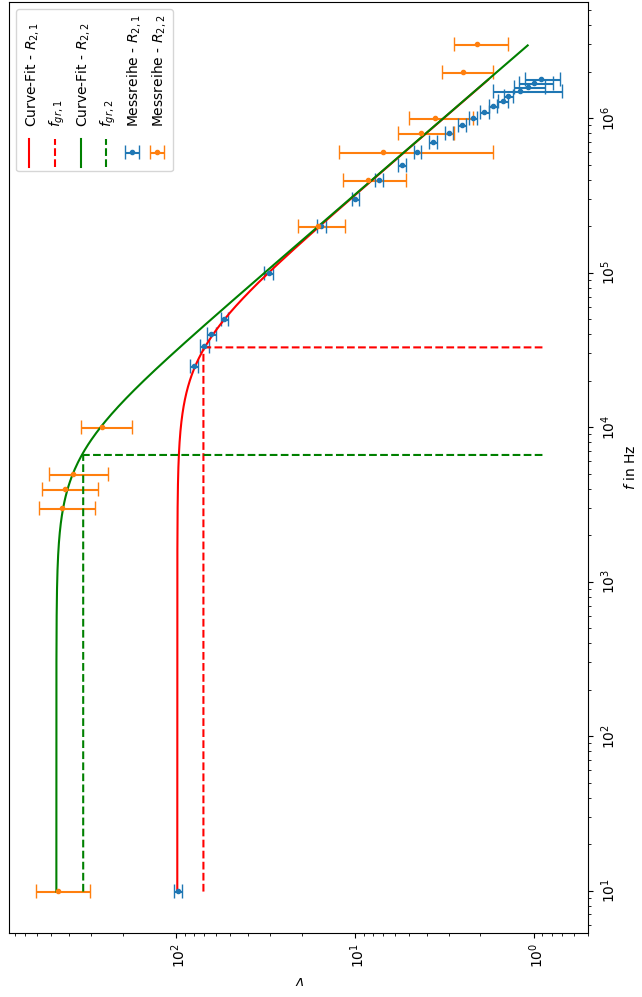
\includegraphics[scale = 0.75]{GegenkopplungMess.PNG}
    \label{abb:invert}
\end{center}


\subsection*{Bandbreite und Flankenabfallzeit}
Die theoretisch erwartete Bandbreite liegt in dem Bereich, in dem die Verstärkung auf das konstante $\frac{\sqrt{2}}{2}$-fache des Maximalwertes gefallen ist. Das heißt für:
\begin{gather}
    R_{2,1}: v_B=\frac{\sqrt{2}}{2}\cdot v_{max}=\frac{\sqrt{2} }{2}\cdot 98=69.296\approx 69\\
    R_{2,2}: v_B=\frac{\sqrt{2}}{2}\cdot v_{max}=\frac{\sqrt{2}}{2}\cdot460 =325.27\approx 325
\end{gather}
Nun soll auch die Beziehung zwischen der Flankenabfallszeit und der Bandbreite B betrachtet werden. Dafür nehmen wir das oben berechnete Verstärkung–Bandbreite–Produkt und setzen dies mit der Transitfrequenz gleich, da die folgende Relation gilt:
\begin{equation}
    f_{gr}=\frac{f_T}{v_{theo}}
\end{equation}
Dadurch bekommen wir folgende Werte für die zwei Widerstände, wobei wir die Transitfrequenz aus einem Datenblatt entnommen haben:
\begin{gather}
    R_{2,1}: f_{gr,1}=\frac{f_T}{v_{t1}}=\frac{4}{100}=0,04\cdot 10^6=40000~\text{Hz}\\
    R_{2,2}: f_{gr,2}=\frac{f_T}{v_{t2}}=\frac{4}{470}=0,0085\cdot 10^6=8500~\text{Hz}
\end{gather}
Da wir den Fehler für die Transitfrequenz aus dem Datenblatt\footnotemark[1] wegen fehlender Angaben weglassen, berechnet sich der Fehler folgendermaßen:
\begin{gather}
    u_{f_{gr,1}}=\sqrt{(\frac{f_T \cdot u_{v_{t1}}}{v_{t1}^2})^2}=0,0016\cdot 10^6=1600~\text{Hz}\\
    u_{f_{gr,2}}=\sqrt{(\frac{f_T \cdot u_{v_{t2}}}{v_{t2}^2})^2}=0,00036\cdot 10^6=360~~\text{Hz}\\
    \Rightarrow \boxed{f_{gr,1}=(40\pm2)~\text{kHz} \tab f_{gr,2}=(8.5\pm0.4)~\text{kHz}}
\end{gather}
Zusätzlich können wir die Grenzfrequenz auch durch folgende Relation berechnen: Wir nehmen an, dass die Beziehung zwischen B und $\tau$ indirekt proportional ist. Dadurch können wir mit folgender Beziehung nach $f_g$ auflösen:
\begin{equation}
    B=2\pi\cdot f_{gr} \Rightarrow \frac{1}{\tau}=B=2\pi\cdot f_{gr} \Leftrightarrow  f_{gr}=\frac{1}{2\pi \tau}
\end{equation}
Dies werden wir nun durch unsere und gemessenen Werte versuchen zu bestätigen und vergleichen dann die verschiedenen Werte für die Grenzfrequenz. \\
Die gemessenen Flankenabfallszeiten haben folgende Werte:
\begin{gather}
    R_{2,1}:\tau_1=\Delta t =4.8~\text{Div} \cdot 0.1~\frac{\mu\text{s}}{div}=4.8\cdot10^{-6}s=4.8~\mu\text{s}\\
    R_{2,2}:\tau_2=\Delta t =4.0~\text{Div} \cdot 0.2~\frac{\mu\text{s}}{\text{Div}}=0-8\cdot10^{-6}s= 0.8~\mu\text{s}\\
    \Rightarrow R_{2,1}: f_{gr,1}=\frac{1}{2\pi \tau_1}= \frac{1}{2\pi \cdot 4.8\cdot 10^{-6}~\text{s}}=33.157~\text{kHz}
\end{gather}
Im Vergleich mit mehreren Gruppen fällt auf, dass wir uns bei $\tau$ von $R_{2,2}=4.7$ M$\Omega$ verschrieben haben. Die Skalierung lag wahrscheinlich bei 5 $\frac{\mu\text{s}}{\text{Div}}$. Daher rechne ich nun mit diesem Wert weiter. 
\begin{gather}
    R_{2,2}: f_{gr,2}=\frac{1}{2\pi \tau_2}= \frac{1}{2\pi \cdot 0.8 \cdot 10^{-6}}=7957.747~\text{Hz}\\
    u_{\tau_1}=\sqrt{0.5^2+(4.8\cdot0.03)^2}\cdot10^{-6}=\cdot10^{-6}=0.52\cdot10^{-6}\\
    u_{\tau_2}=\sqrt{0.1^2+(20\cdot0.03)^2}\cdot10^{-6}=0.608\cdot10^{-6}\\
    u_{f_{gr,1}}=\sqrt{(\frac{u_{\tau_1}}{\tau^2 \cdot 2\pi})^2}= 3592.04\\
    u_{f_{gr,2}}=\sqrt{(\frac{u_{\tau_2}}{\tau^2 \cdot 2\pi})^2}= 241.9\\
    \Rightarrow\boxed{
    f_{gr,1}=(33\pm4)~\text{kHz} \tab f_{gr,2}=(8.0\pm0.2)~\text{kHz}
    }
\end{gather}
Beim Vergleichen der auf zwei Arten berechneten Grenzfrequenzen $f_{gr}$ bemerkt man, dass sie deutlich in der gleichen Größenordnung sind und vor allem die Werte für den Widerstand $R_{2,2}=4.7 $ M$\Omega$ sich in ihren Fehlern deutlich überschneiden. Auch bei dem anderen Widerstand merkt man, dass sich die Werte stark annähern, sich aber nicht in den Fehlern überschneiden. Dafür könnten mehrere Gründe die Ursache sein. Zum Einen könnten es Messunsicherheiten, zu lange Kabel oder ähnliche Schalttechnische Fehler sein. Dies würde jedoch auch einen Fehler bei dem anderen Widerstand hervorrufen, was es jedoch wie gerade beschrieben nicht macht. Ein anderer Grund könnten fehlerhafte Mitschriften der Protokollperson sein. Da dies auch bei dem anderen Widerstand vorgekommen ist, ist dies auch hier nicht ausgeschlossen. Jedoch ist die Abweichung sehr gering, weshalb man es auch der generellen Ableseungenauigkeit zu schieben könnte. \\
Im Allgemeinen erkennt man jedoch, dass beide Rechenmethoden zu einem sehr ähnlichen Ergebnis führen, wodurch unsere theoretische Vermutung der Indirekten Proportionalität von B zu $\tau$ bestätigt wurde.\\
\newline
Abschließend ist noch anzumerken, dass die Werte für $b$ unseres Fits aus dem zweiten Teil dieses Kapitels tatsächlich den jeweiligen Grenzfrequenzen $f_{gr,i}$ entsprechen kann, da diese in der korrekten Größenordnung wie oben berechnet vorhanden sind.
\newpage